\documentclass{article}
% --- watermark (auto-inserted) ---
\usepackage{xcolor}
\usepackage{xfp}% \fpeval; in the kernel since 2022, harmless on older LaTeX
\usepackage{draftwatermark}
\newlength{\watermarkTextWidth}
\AddToHook{begindocument/end}{%
  \SetWatermarkText{\normalfont Generated by The Agentic Scientist}%
  \SetWatermarkFontSize{10pt}%
  \SetWatermarkLightness{0.85}%
  \settowidth{\watermarkTextWidth}{\normalfont\fontsize{10pt}{12pt}\selectfont Generated by The Agentic Scientist}%
  \edef\watermarkScale{\fpeval{0.8 * sqrt(\paperwidth**2 + \paperheight**2) / \watermarkTextWidth}}%
  \edef\watermarkAngle{\fpeval{atand(\paperheight/\paperwidth)}}%
  \SetWatermarkScale{\watermarkScale}%
  \SetWatermarkAngle{\watermarkAngle}%
}
% --- end watermark ---

\usepackage{iclr2026_conference,times}
\usepackage{amsmath,amssymb,booktabs,longtable,graphicx,subcaption}
\usepackage{hyperref,url}
\title{Memorization Without Observed Grokking Across MLP Widths}
\author{}
\newcommand{\TM}{T_{\mathrm{M}}}
\newcommand{\TG}{T_{\mathrm{G}}}
\newcommand{\LH}{L_H}

\begin{document}
\maketitle

\begin{abstract}
Does increasing model size change delayed generalization, or only the speed of fitting the training data? We study this distinction in full-batch ReLU multilayer perceptrons on modular addition and subtraction. A fixed learning-rate protocol crosses three hidden widths with two AdamW weight-decay settings and three initialization seeds, producing 36 completed training records. Memorization and generalization are defined by separate sustained accuracy thresholds. Within 20,000 updates, 30 records attain memorization but none attains generalization. Wider networks fit earlier without decay and fit where the narrowest networks fail with positive decay; these differences do not establish faster grokking. An audit of the reported endpoint-substituted lag shows that its positive 500-update width contrast, including a degenerate seed interval, follows from fitting times and censoring rather than observed generalization. The evidence supports a finite-horizon separation between width-dependent fitting and unobserved generalization, while leaving the eventual dependence of grokking time on model size unidentified.
% @evidence[[paper_data.json#/final_evaluation/evaluation_evidence/episodes]]
% @evidence[[paper_data.json#/final_evaluation/metrics/width_lag_contrast]]
\end{abstract}

\section{Introduction}

Small algorithmic datasets offer an unusually transparent setting for investigating generalization: the target rule is known, every possible input can be enumerated, and training performance can be separated from performance on unseen inputs. Yet fitting such data need not reveal when a network learns the underlying operation. Grokking names the striking case in which generalization emerges long after the training data have been fitted \citep{Power2022GrokkingGB}. This separation raises a basic question about scale: does a larger network change the arrival of generalization, or simply change the point from which the delay is measured?

The distinction matters because a delay is a difference between event times. Earlier memorization can increase a measured delay even if generalization is unchanged. Conversely, replacing an unobserved generalization event with the training endpoint can produce an apparently precise contrast without any generalization event having occurred. A study of model size therefore needs to report fitting, generalization, and non-attainment separately, rather than infer one from another. Training accuracy alone is particularly inadequate as a proxy for learning an algorithm; the broader distinction between finite-sample fitting and useful generalization is well established \citep{Zhang2017Rethinking}.

We examine a controlled width-by-decay grid for a single fixed optimization recipe on addition and subtraction modulo 97. The models are one-hidden-layer ReLU networks with concatenated one-hot inputs. Hidden width varies over 16, 64, and 256; all other architectural choices are fixed. Two decay settings and three initialization seeds give 36 training records. Our working explanation is deliberately limited: width may remove a fitting bottleneck without making generalization observable within the same computational horizon. A stronger claim, that width changes an eventual generalization clock, requires events that this study does not observe.
% @evidence[[paper_data.json#/final_evaluation/evaluation_evidence/episodes]]
% @evidence[[source_evidence/evaluate_final.py#L656-L660]]
% @evidence[[source_evidence/evaluate_final.py#L789-L871]]

The results make this separation concrete. All wider networks attain sustained memorization at the first noninitial checkpoint. Narrow networks fit later without decay and do not attain memorization with positive decay. Nevertheless, no condition reaches sustained held-out accuracy of 95\% within 20,000 updates. Thus, the observed size dependence is a fitting result, not an estimate of the size dependence of grokking time.
% @evidence[[paper_data.json#/final_evaluation/evaluation_evidence/episodes]]

Our contributions are an explicit finite-horizon width comparison across related modular operations, a complete seed-level account of fitting and generalization non-attainment, and an algebraic audit of an endpoint-substituted lag statistic. We show why a nonzero width contrast and a zero-width seed interval can coexist with no observed generalization. These findings delimit what the evaluated configuration establishes; they neither rule out later grokking nor choose among proposed neural mechanisms.
% @evidence[[paper_data.json#/final_evaluation/metrics/width_lag_ci_low]]
% @evidence[[paper_data.json#/final_evaluation/metrics/width_lag_ci_high]]

\begin{figure}[t]
  \centering
  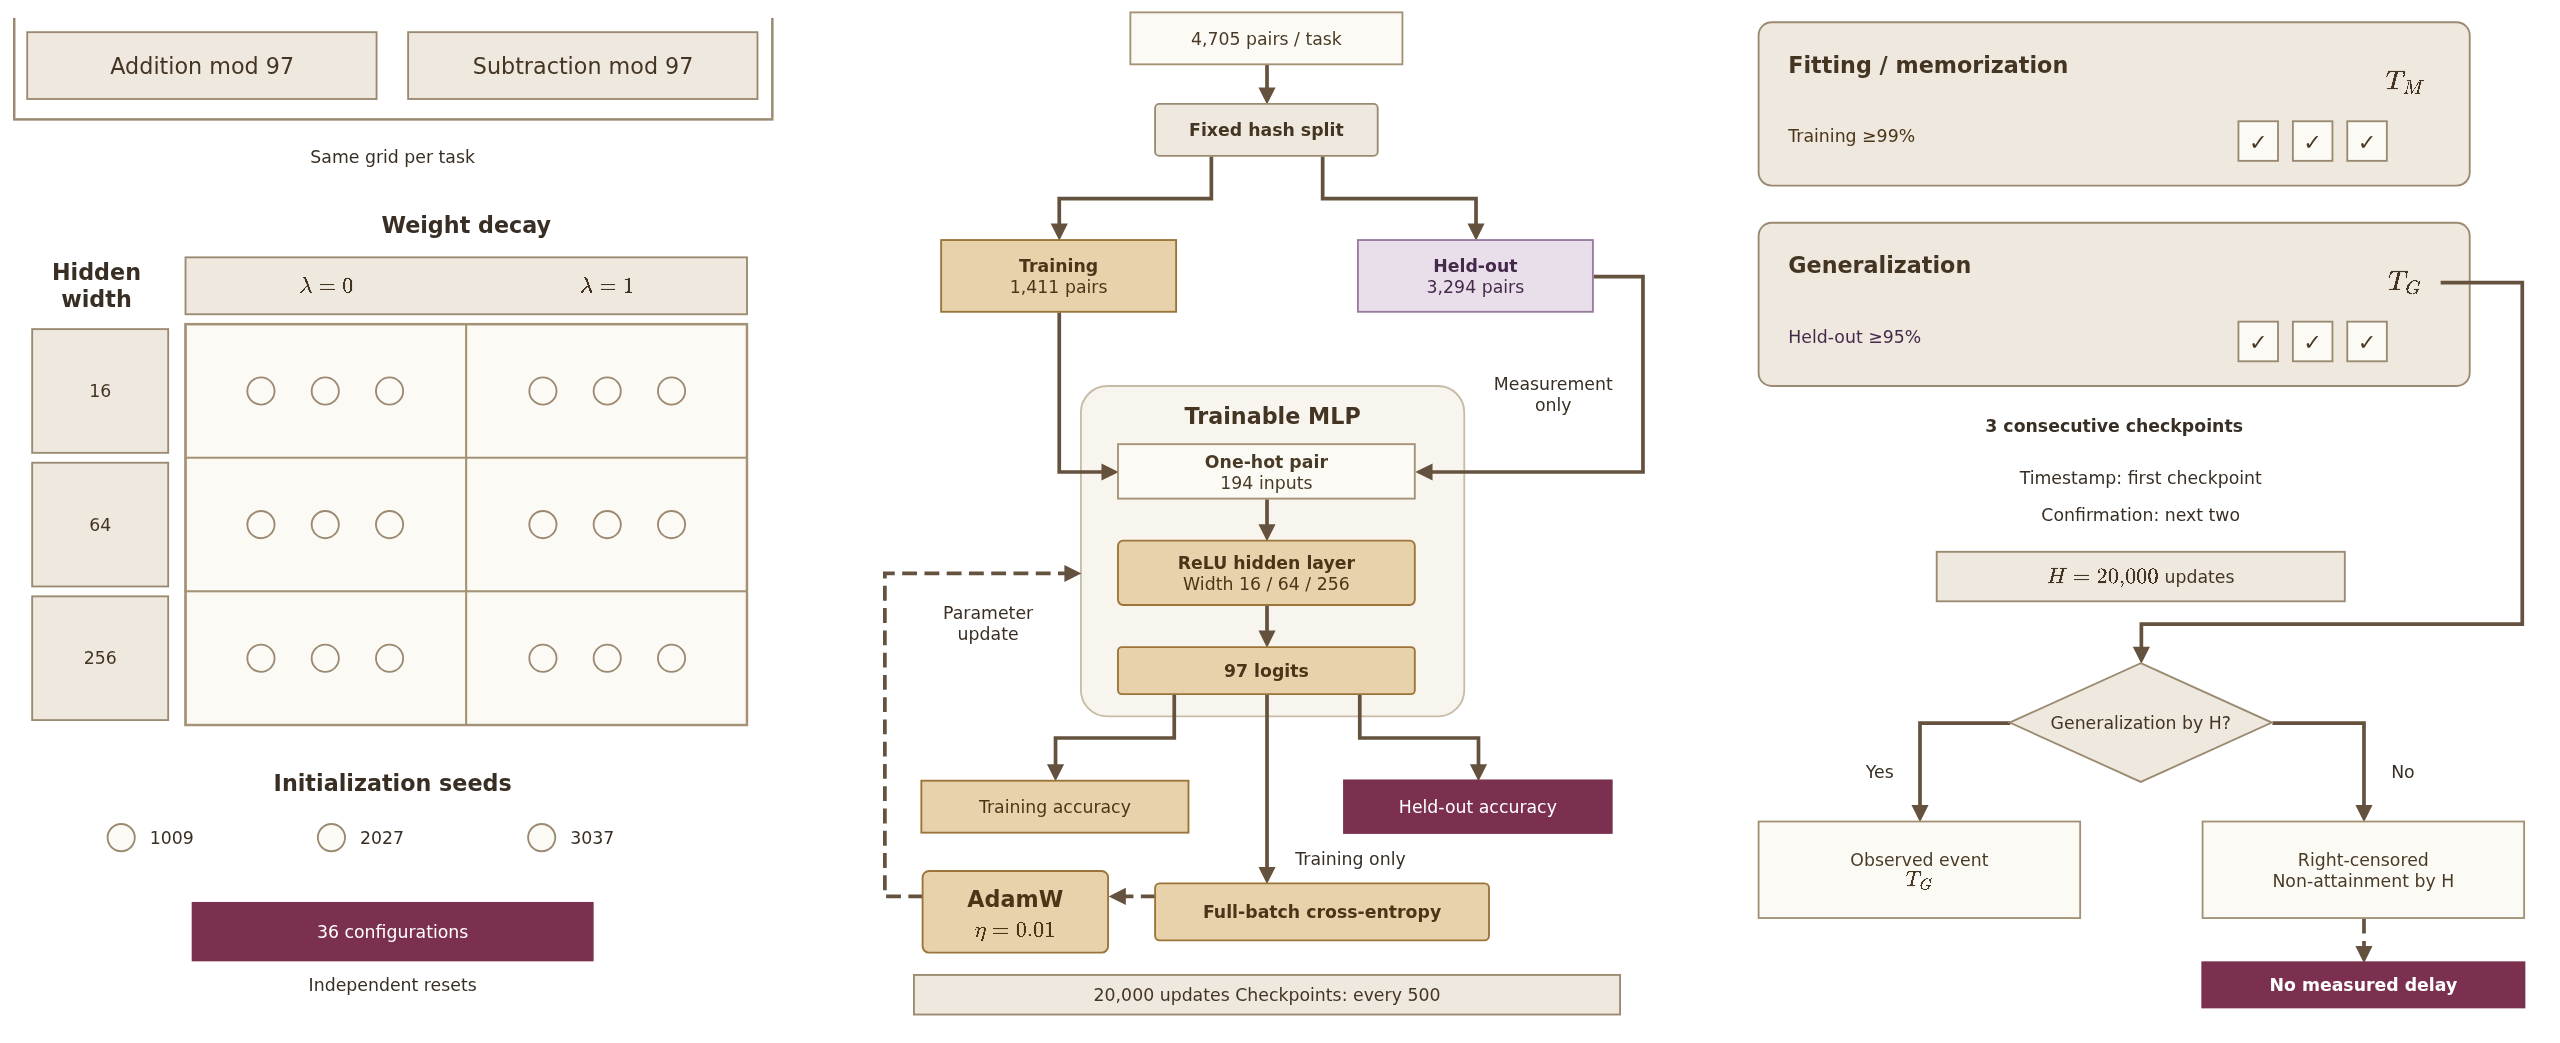
\includegraphics[width=\textwidth]{figures/study_overview.png}
  \caption{Study design and observation boundary. Addition and subtraction modulo 97 are evaluated under a shared fixed-rate MLP protocol crossing three hidden widths, two weight-decay settings, and three initialization seeds. Memorization requires training accuracy of at least 99\%; generalization requires held-out accuracy of at least 95\%, each for three consecutive checkpoints. Non-attainment at 20,000 updates is not a measured generalization delay. The diagram summarizes the design, not a proposed neural circuit.}
  \label{fig:overview}
  % @evidence[[paper_data.json#/final_evaluation/evaluation_evidence/episodes]]
  % @evidence[[source_evidence/evaluate_final.py#L721-L743]]
\end{figure}

\section{Related Work}

\paragraph{Grokking and candidate explanations.}
\citet{Power2022GrokkingGB} establish delayed generalization on small algorithmically generated datasets and describe its dependence on dataset size. Our experiment uses this setting to distinguish finite-budget fitting from generalization-event timing; it is not a replication of a particular delayed-generalization trajectory. \citet{Liu2023Omnigrok} relate grokking to training and test loss landscapes as a function of weight norm and demonstrate its presence beyond algorithmic data. \citet{Varma2023ExplainingGT} propose competition between faster memorizing solutions and more norm-efficient generalizing solutions. \citet{Kumar2024LazyRich} analyze a transition from lazy to feature-learning dynamics, including a two-layer polynomial-regression setting. These explanations motivate keeping optimization, regularization, and representation effects distinct. Our recorded norms and losses do not measure circuit efficiency or a lazy-to-rich transition, and cannot discriminate these accounts.

\paragraph{Capacity and generalization need not move together.}
\citet{Zhang2017Rethinking} demonstrate that fitting training labels and explaining generalization are different problems. \citet{Nakkiran2020DoubleDescent} show that increasing model size or training duration need not yield monotone test performance. \citet{Davies2023Unifying} propose a common pattern-learning-speed perspective on grokking and double descent, including variation in capacity. This context cautions against treating a width effect on training accuracy as sufficient evidence about held-out learning. Our grid is too sparse, and its accuracies too uniformly low, to establish a double-descent curve or a general capacity law.

\paragraph{Regularization and the role of the learning rate.}
AdamW decouples weight decay from the loss-gradient update \citep{Loshchilov2017DecoupledWD}. However, its per-update parameter shrinkage still depends on the learning rate used in that update. We therefore compare decay arms under one shared constant rate rather than interpret a change in the learning-rate recipe as a clean intervention on decay alone. The literature discussion is restricted to exact, permitted starter sources; we make no exhaustive priority or novelty claim from this restricted coverage.

\section{Method}
\label{sec:method}

\subsection{Problem, Data, and Evaluation Target}

For a pair $(a,b)\in\{0,\ldots,p-1\}^2$, the target is either $(a+b)\bmod p$ or $(a-b)\bmod p$, with $p=97$. Each operation has $p^2=9,409$ possible ordered pairs. The final evaluation uses a deterministic subset of 4,705 pairs for each operation, with 1,411 training pairs and 3,294 held-out pairs. Thus the training set is approximately 30\% of the retained subset, not 30\% of the entire operation table; it covers approximately 15\% of all possible inputs. Addition and subtraction use independently constructed operation-specific partitions.
% @evidence[[paper_data.json#/final_evaluation/evaluation_evidence/episodes]]
% @evidence[[source_evidence/evaluate_final.py#L588-L613]]
% @evidence[[source_evidence/resources/final/benchmark.json]]

The partition is reproducible without downloading data. Each input and operation are encoded in canonical JSON, normalized, and hashed. Sorting the hashes separates the development subset from the final subset. A second hash ordering with a fixed training prefix assigns the training portion within the final subset. The split is fixed across initialization seeds and widths. Consequently, seed variability measures training-initialization variability on a fixed split, not uncertainty over fresh data partitions. The held-out set is used for recording performance, not for gradient updates. Appendix~\ref{app:construction} specifies the construction and readable source locations.
% @evidence[[source_evidence/evaluate_final.py#L588-L631]]
% @evidence[[source_evidence/evaluate_final.py#L825-L870]]

We report both operations rather than treating subtraction as an unseen transfer task. Each network is independently trained from scratch on its own operation. The shared architecture and optimization recipe permit a condition-specific replication of the width comparison, but not a claim of cross-task representation transfer.
% @evidence[[paper_data.json#/final_evaluation/evaluation_evidence/episodes]]
% @evidence[[source_evidence/evaluate_final.py#L656-L660]]

\subsection{Working Explanation and Falsifiable Predictions}

The working explanation separates \emph{fitting capacity under the chosen optimizer} from \emph{learning a held-out algorithm}. Increasing width can make the finite training table easier to fit without supplying evidence that the network acquires the arithmetic rule. In a regularized setting, the fitting requirement may become more demanding, so that the narrowest network no longer attains the same training criterion even though wider networks do. This is an explanation of operational fitting behavior, not a claim that parameter count alone determines representational capacity.

The corresponding finite-horizon predictions are explicit. At fixed decay, wider networks should attain the training criterion no later than the narrowest model, or attain it where the narrowest does not. If increased width is sufficient to reveal delayed generalization in this protocol, at least one wider condition should additionally cross the held-out criterion within the budget. The former prediction can be checked using fitting events; the latter can be falsified for this particular horizon. An eventual equality, ordering, or equivalence of generalization times cannot be tested unless those times are observed or otherwise bounded more informatively. These are interpretive predictions for the retained design, not a claim of preregistration or an independent confirmatory test.

\subsection{Width and Decay Comparisons}

The input vector is $x=[e_a;e_b]\in\mathbb{R}^{194}$, a concatenation of two one-hot encodings. The classifier is
\begin{equation}
 f_\theta(a,b)=W_2\operatorname{ReLU}(W_1x+b_1)+b_2\in\mathbb{R}^{97}.
\end{equation}
The hidden width $w\in\{16,64,256\}$ gives $292w+97$ trainable parameters: 4,769, 18,785, and 74,849, respectively. Both linear layers have biases. The implementation uses the default PyTorch linear-layer initialization without a width-specific logit-scale calibration. Therefore, the comparison holds the layer family fixed but does not isolate width from all initialization-scale effects.
% @evidence[[paper_data.json#/final_evaluation/evaluation_evidence/episodes]]
% @evidence[[source_evidence/evaluate_final.py#L802-L850]]

Each condition minimizes full-batch cross-entropy with AdamW. The fixed learning rate is $\eta=0.01$ throughout training; weight decay is $\lambda\in\{0,1\}$, with optimizer coefficients $(0.9,0.999)$ and numerical constant $10^{-8}$. All model parameters are passed to the same optimizer without separate bias exclusions. The recipe controller exposes only a bounded open-loop schedule and receives no training metrics. Its evaluated constant-rate setting is identical across operations, widths, decays, and seeds. The frozen controller and evaluator, rather than proposal descriptions, define the implemented method.
% @evidence[[source_evidence/controller/src/program.py#L46-L78]]
% @evidence[[source_evidence/evaluate_final.py#L842-L870]]

For constant $\eta$, the multiplicative shrinkage contribution of AdamW alone is $(1-\eta\lambda)^t$ after $t$ updates. This algebra explains why changing a learning-rate recipe would change both gradient updates and accumulated shrinkage. It does not predict the norm or accuracy of the trained network, whose gradient contributions are not removed. We do not compare the fixed recipe empirically against the original lower-rate configuration because no matched final evaluation of that configuration is retained. Nor do we reinterpret development scores as final-task measurements.
% @evidence[[source_evidence/controller/src/EXPERIMENT_SCOPE.md]]
% @evidence[[source_evidence/evaluate_final.py#L846-L870]]

\subsection{Training Protocol and Sustained Events}

The evaluation crosses two operations, three widths, two decay values, and seeds 1009, 2027, and 3037. Training runs for $H=20,000$ full-batch updates, with an initial measurement and measurements every 500 updates. The worker uses deterministic PyTorch algorithms, one compute thread, and one interoperation thread. Each condition resets the model and optimizer; no weights are transferred between conditions. The environment specifies NumPy 2.1.3 and PyTorch 2.5.1+cpu. Source evidence, dependencies, and output-to-script mappings are included with the supplementary material.
% @evidence[[paper_data.json#/final_evaluation/evaluation_evidence/episodes]]
% @evidence[[source_evidence/evaluate_final.py#L789-L799]]
% @evidence[[source_evidence/requirements.txt]]

Let $A_{\mathrm{tr}}(t)$ and $A_{\mathrm{ho}}(t)$ denote checkpoint accuracies. We define $\TM$ as the first checkpoint whose training accuracy and next two checkpoint accuracies all reach 99\%. Likewise, $\TG$ uses a held-out threshold of 95\%. A recorded crossing is timestamped at the start of the sustained sequence, although it is confirmed only after observing the following checkpoints. Events near the endpoint without sufficient confirming measurements do not satisfy the rule. These operational event times are checkpoint-resolved, not continuous measurements of the underlying transition.
% @evidence[[source_evidence/evaluate_final.py#L721-L743]]
% @evidence[[paper_data.json#/final_evaluation/evaluation_evidence/episodes]]

Late-window accuracy averages the final five checkpoints, from 18,000 through 20,000 updates. It is a descriptive endpoint summary and is not interchangeable with either sustained-event criterion. We preserve all completed records, including fitting failures and held-out non-attainment. All 36 records complete, so the results contain neither missing trajectories nor a denominator restricted to fitting-capable models. No new training is performed for this paper; the figures and tables recompute summaries from the sealed final observations.
% @evidence[[paper_data.json#/final_evaluation/evaluation_evidence/episodes]]
% @evidence[[paper_data.json#/final_evaluation/metrics/completion_fraction]]

\subsection{Capped Lag and Statistical Reporting}
\label{sec:lag}

To audit the retained lag summary, we reproduce its exact definition:
\begin{equation}
\LH=\begin{cases}
H,&\TM\text{ unobserved},\\
\max\{0,\min(\TG,H)-\TM\},&\TM\text{ observed},
\end{cases}
\label{eq:lag}
\end{equation}
where an unobserved $\TG$ is replaced by $H$. This is an administratively capped statistic, not an uncensored grokking time. In particular, assigning $H$ when memorization is unobserved does not define a genuine post-memorization waiting time. When memorization is observed but generalization is not, $H-\TM$ is the observed waiting period without an attained event.
% @evidence[[source_evidence/evaluate_final.py#L728-L743]]

For seed $s$ and decay $\lambda$, the paired extreme-width contrast averages over operations:
\begin{equation}
D_s(\lambda)=\frac{1}{2}\sum_{o\in\{+, -\}}
\big[\LH(o,16,\lambda,s)-\LH(o,256,\lambda,s)\big].
\label{eq:contrast}
\end{equation}
We reproduce the supplied mean and Student-$t$ interval across the three paired seed contrasts, as well as the difference of mean contrasts between decay arms. All individual seeds are shown in the plots, and descriptive means and sample standard deviations are used where appropriate. The checkpoints, operations, and decay arms are not treated as independent replications. With no generalization events, we do not estimate a distribution of eventual generalization times or infer a population event probability from the pooled 36 conditions.
% @evidence[[source_evidence/evaluate_final.py#L746-L773]]
% @evidence[[paper_data.json#/final_evaluation/evaluation_evidence/episodes]]

\section{Results}

\subsection{Width Changes Fitting, but Generalization Is Not Observed}

Table~\ref{tab:events} reports every condition's seed-specific memorization times. With zero decay, all networks memorize: width 16 reaches the sustained criterion at 1,000--1,500 updates, whereas widths 64 and 256 do so at 500 updates in both operations and every seed. The wider conditions are indistinguishable at this checkpoint resolution. Their common event timestamp means they satisfy the rule from the first noninitial checkpoint onward, not that their underlying fitting transitions occur at exactly the same update.
% @evidence[[paper_data.json#/final_evaluation/evaluation_evidence/episodes]]

Positive decay changes the narrowest condition qualitatively. All six width-16 records fail to attain sustained memorization by the horizon; every width-64 and width-256 record still attains it at 500 updates. Across the entire grid, 30 of 36 records memorize, but no record attains sustained generalization. There are therefore no observed delayed-generalization events, including among the 30 fitting-capable records. The completed evaluation supports a negative finite-horizon result, rather than a comparison of observed grokking times.
% @evidence[[paper_data.json#/final_evaluation/evaluation_evidence/episodes]]
% @evidence[[paper_data.json#/final_evaluation/metrics/delayed_fraction]]

\begin{table}[t]
  \centering
  \small
  % @evidence[[paper_data.json#/final_evaluation/evaluation_evidence/episodes]]
\begin{tabular}{llrrrrr}
\toprule
Operation & $\lambda$ & Width & $T_M^{(1009)}$ & $T_M^{(2027)}$ & $T_M^{(3037)}$ & $G$ observed \\
\midrule
Addition & 0 & 16 & 1,500 & 1,000 & 1,000 & 0/3 \\
Addition & 0 & 64 & 500 & 500 & 500 & 0/3 \\
Addition & 0 & 256 & 500 & 500 & 500 & 0/3 \\
Addition & 1 & 16 & \textemdash & \textemdash & \textemdash & 0/3 \\
Addition & 1 & 64 & 500 & 500 & 500 & 0/3 \\
Addition & 1 & 256 & 500 & 500 & 500 & 0/3 \\
Subtraction & 0 & 16 & 1,000 & 1,000 & 1,000 & 0/3 \\
Subtraction & 0 & 64 & 500 & 500 & 500 & 0/3 \\
Subtraction & 0 & 256 & 500 & 500 & 500 & 0/3 \\
Subtraction & 1 & 16 & \textemdash & \textemdash & \textemdash & 0/3 \\
Subtraction & 1 & 64 & 500 & 500 & 500 & 0/3 \\
Subtraction & 1 & 256 & 500 & 500 & 500 & 0/3 \\
\bottomrule
\end{tabular}

  \caption{Sustained memorization times in updates, with generalization attainment shown separately. A dash denotes no sustained memorization by 20,000 updates, not a missing or unfinished record. The final column counts observed sustained generalization events across the three seeds. Every condition has a complete trajectory.}
  \label{tab:events}
  % @evidence[[paper_data.json#/final_evaluation/evaluation_evidence/episodes]]
\end{table}

Figure~\ref{fig:outcomes} complements the event table with late-window accuracies. Without decay, all training accuracies average 100\%. With positive decay, the width-16 averages are 56.664\% for addition and 55.625\% for subtraction; all wider conditions average 100\%. Thus the narrow-model non-attainment is not merely a transient miss of a threshold close to perfect fitting. It is accompanied by much lower training accuracy in the recorded late window.
% @evidence[[paper_data.json#/final_evaluation/evaluation_evidence/episodes]]
% @evidence[[analysis/derived_results.json#/conditions]]

\begin{figure}[t]
  \centering
  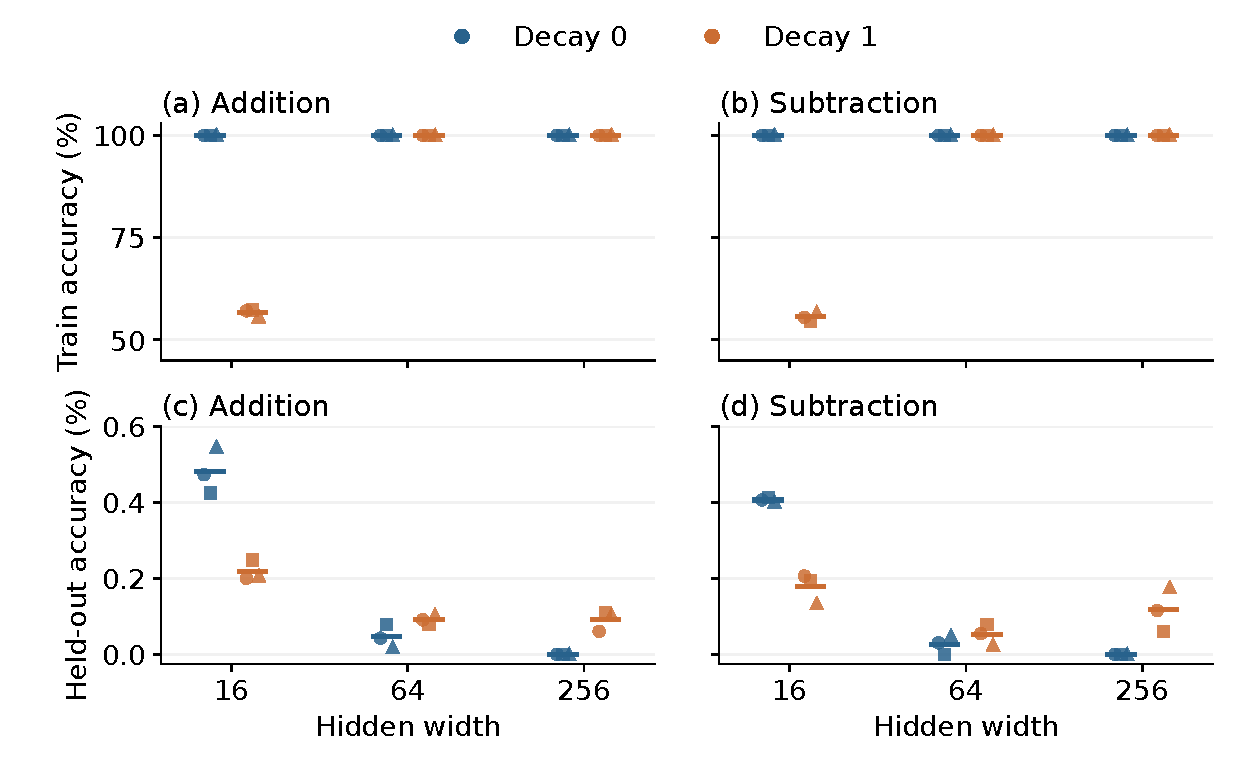
\includegraphics[width=\textwidth]{figures/width_decay_outcomes.pdf}
  \caption{Late-window fitting and held-out accuracy separate sharply. Panels (a,b) show training accuracy; (c,d) show held-out accuracy, with a separate shared scale for each row. Values average the final five checkpoints. Colors encode decay; circles, squares, and triangles identify seeds 1009, 2027, and 3037, respectively. Short horizontal bars are condition means, not uncertainty intervals. The training axis is restricted to expose the narrow positive-decay fitting deficit; held-out accuracy remains far below the sustained generalization threshold in every condition.}
  \label{fig:outcomes}
  % @evidence[[paper_data.json#/final_evaluation/evaluation_evidence/episodes]]
\end{figure}

\subsection{Held-Out Accuracy Does Not Track Earlier Fitting}

The zero-decay width-16 models have mean late-window held-out accuracies of $0.482\pm0.061$\% for addition and $0.407\pm0.006$\% for subtraction, where the uncertainty shown is the sample standard deviation across initialization seeds. At width 64 these means fall to 0.047\% and 0.026\%, respectively; at width 256 they are zero in all seeds. These measurements contradict a monotone improvement in endpoint accuracy with width for this decay arm. They do not establish a general law that larger models generalize worse.
% @evidence[[paper_data.json#/final_evaluation/evaluation_evidence/episodes]]
% @evidence[[analysis/derived_results.json#/conditions]]

With positive decay, mean held-out accuracies for widths 16, 64, and 256 are 0.219\%, 0.091\%, and 0.091\% on addition, and 0.178\%, 0.053\%, and 0.117\% on subtraction. The variation is not a common monotone width trend across arms. More importantly, none of these small differences approaches the generalization criterion. The evidence supports a distinction between fitting attainment and useful held-out learning, not a superiority claim for a particular width. Full seed values appear in the supplement rather than being hidden behind condition averages.
% @evidence[[paper_data.json#/final_evaluation/evaluation_evidence/episodes]]
% @evidence[[analysis/derived_results.json#/conditions]]

The mean late-window held-out accuracy over all conditions is 0.142515\%. The stored reference predictors average 0.865209\% for a training-label-mode predictor, 0.865209\% for a lookup-with-mode-fallback predictor, 0.949201\% for label-deranged prediction alignment, and 1.050732\% for the initialized network. The trained networks' mean gap to these four references is $-0.790073$ percentage points. This is a descriptive comparison to these particular references, not a test against independent random-label training. The lookup reference necessarily duplicates the mode predictor on disjoint held-out input pairs, so the reference average does not represent four independent controls.
% @evidence[[paper_data.json#/final_evaluation/metrics/control_gap]]
% @evidence[[paper_data.json#/final_evaluation/evaluation_evidence/episodes]]
% @evidence[[source_evidence/evaluate_final.py#L805-L847]]

\subsection{Loss and Norm Diagnostics Qualify the Accuracy Comparison}

Endpoint loss provides a complementary view of the poor held-out predictions. On addition at width 16, mean final-checkpoint held-out cross-entropy is 339.459 without decay and 8.390 with positive decay. At width 256, the corresponding values are 89.877 and 8.627. Thus, a decay setting can substantially reduce held-out cross-entropy without producing sustained generalization, and its ranking by loss need not match its ranking by top-one accuracy. These are comparisons between the evaluated configurations, not evidence that reduced loss must precede an eventual transition. The full endpoint table is provided in the supplement.
% @evidence[[paper_data.json#/final_evaluation/evaluation_evidence/episodes]]
% @evidence[[analysis/derived_results.json#/records]]

The initial parameter norm also differs across widths: averaging the three seeds gives 6.288, 7.383, and 10.904 for widths 16, 64, and 256. These norms are the same across operations and decay arms at a fixed width and seed, because initialization is reset before each condition. This check supports comparability of decay arms at initialization while making clear that widths are not norm-matched. An initial norm difference is not itself a difference in functional logit scale, and neither quantity establishes a particular learning regime. The retained diagnostics therefore sharpen the implementation boundary without resolving the mechanism.
% @evidence[[paper_data.json#/final_evaluation/evaluation_evidence/episodes]]
% @evidence[[source_evidence/evaluate_final.py#L805-L850]]

\subsection{A Precise Capped-Lag Contrast Without Generalization Events}

Figure~\ref{fig:censoring} shows the capped statistic rather than labeling it as observed delay. Since all generalization events are unobserved, every fitted record has $\LH=H-\TM$. Under positive decay, width 16 receives the special non-memorization value 20,000, while width 256 receives $20,000-500=19,500$. Their paired contrast is therefore 500 updates for every seed and both operations. The supplied three-seed interval is $[500,500]$ updates because these recorded contrasts have zero sample variation. Its degeneracy reflects the endpoint rule and checkpoint-aligned fitting events, not precise knowledge of generalization time.
% @evidence[[paper_data.json#/final_evaluation/evaluation_evidence/episodes]]
% @evidence[[paper_data.json#/final_evaluation/metrics/width_lag_contrast]]
% @evidence[[paper_data.json#/final_evaluation/metrics/width_lag_ci_low]]
% @evidence[[paper_data.json#/final_evaluation/metrics/width_lag_ci_high]]

\begin{figure}[t]
  \centering
  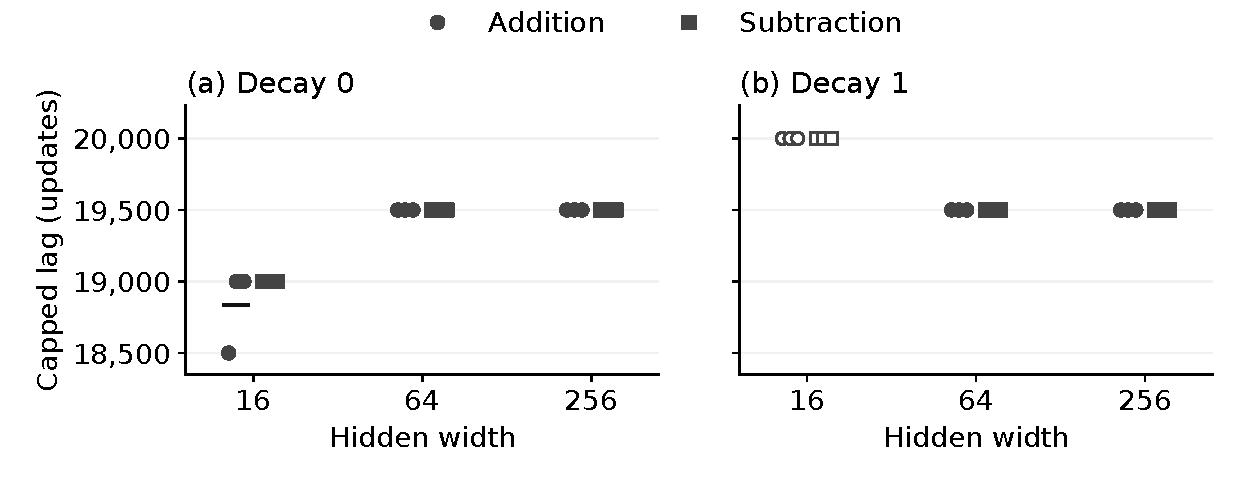
\includegraphics[width=\textwidth]{figures/censoring_audit.pdf}
  \caption{Administrative endpoint substitution determines the displayed lag. Circles denote addition and squares subtraction; horizontal bars are condition means. Filled symbols indicate observed memorization; hollow symbols indicate memorization non-attainment. All generalization events are unobserved. The focused vertical range does not begin at zero. In panel (a), earlier fitting at larger widths increases $H-\TM$. In panel (b), the hollow width-16 observations instead receive the special value $H$, creating a positive narrow-minus-wide contrast without any observed generalization event.}
  \label{fig:censoring}
  % @evidence[[paper_data.json#/final_evaluation/evaluation_evidence/episodes]]
\end{figure}

Without decay, the three operation-averaged narrow-minus-wide contrasts are $-750$, $-500$, and $-500$ updates, averaging $-583.333$. Here every model memorizes, and the wider models have \emph{larger} capped lags precisely because they fit earlier. The difference between the decay-arm mean contrasts is 1,083.333 updates. The overall capped-lag mean is 19,486.111 updates. Neither quantity estimates a difference in observed grokking times. A sign change across arms is possible simply because the special rule for missing memorization replaces the ordinary post-fitting waiting period.
% @evidence[[paper_data.json#/final_evaluation/metrics/decay_interaction]]
% @evidence[[paper_data.json#/final_evaluation/metrics/restricted_mean_lag]]
% @evidence[[paper_data.json#/final_evaluation/evaluation_evidence/episodes]]

This audit also limits the working explanation. The fitting prediction is borne out within the measured grid. The proposition that wider networks suffice to reveal delayed generalization within this budget is not supported. However, the data cannot establish equal eventual generalization times across widths, nor that any of the fitted models will ever generalize. Administrative censoring preserves a finite observation window; it does not manufacture the missing event.

\section{Discussion and Limitations}

\paragraph{What the width comparison identifies.}
The cleanest result is conditional: under the same representation, optimizer recipe, data partition, and update budget, changing width changes fitting behavior without yielding a generalization event. The decay comparison likewise identifies differences between evaluated configurations, not an isolated mechanism of representational capacity. Default initialization, parameterization, and optimization interact with width. A claim that width alone changes the efficiency of a memorizing circuit would require additional measurements and controls that are not present.

\paragraph{Why this is not a generalization-time law.}
The sustained definition prevents a transient checkpoint excursion from being reported as stable attainment, but its temporal resolution is limited and its required confirmation shortens the window for detectable late events. Extending training could change the qualitative outcome. Conversely, continued low held-out accuracy could persist without contradiction. The retained trajectories give neither outcome. The capped statistic is useful only when read alongside the two event indicators; reporting it alone would erase the distinction between failing to fit and fitting without generalization.

\paragraph{Mechanistic explanations remain open.}
There are no independently trained random-label controls, matched initial logit-scale interventions, norm-matched comparisons, circuit decompositions, or kernel/feature-learning measurements. Weight norm and loss are recorded, but they do not identify which of the candidate explanations in related work applies. In particular, the absence of an observed transition does not show that norm efficiency, lazy-to-rich learning, or a delayed representation change is absent. Nor can the poor endpoint accuracy identify a unique failure cause. We therefore do not attribute the result to an unmeasured circuit or diagnose an adaptivity or validity failure from performance alone.
% @evidence[[source_evidence/controller/src/EXPERIMENT_SCOPE.md]]
% @evidence[[paper_data.json#/final_evaluation/evaluation_evidence/episodes]]

\paragraph{Update budget is not compute matching.}
All conditions receive the same number of full-batch optimizer updates and the same checkpoint schedule, making the event comparison interpretable in update units. Equal updates do not imply equal arithmetic work or equal wall-clock cost across widths. The retained timing fields summarize seed-level evaluations rather than isolated, hardware-controlled per-width throughput. Consequently, earlier fitting in update units is not a measured speedup per CPU second or a resource-efficiency claim. The study also fixes one learning-rate recipe instead of tuning a separate optimum for each width. Its negative generalization result applies to that shared recipe, not to the best achievable performance of every model size.
% @evidence[[paper_data.json#/final_evaluation/evaluation_evidence/episodes]]
% @evidence[[source_evidence/controller/src/program.py]]

\paragraph{Coverage and uncertainty.}
The empirical scope is one modulus, one input representation, one hidden-layer family, three widths, two decay values, three initialization seeds, and a fixed split per operation. The operations are closely related, not a representative distribution of algorithmic tasks. The small seed count limits uncertainty assessment; the paired interval pertains only to the implemented capped summary and does not incorporate split variation or hyperparameter selection. We do not pool checkpoint measurements into extra replications, infer confidence from overlapping seed markers, or interpret a zero-width interval as robustness across unseen settings. Reusing a seed aligns the random-number initialization procedure, but differently shaped networks do not have identical initial functions. Likewise, the two operations share an algebraic family while having different fixed input partitions. Pairing improves the definition of a conditional comparison; it does not turn those observations into independent draws from a broad population of models or tasks.
% @evidence[[paper_data.json#/final_evaluation/evaluation_evidence/episodes]]

\paragraph{Configuration and evidence boundaries.}
The final factorial evaluates one fixed learning-rate recipe. The absence of a matched final result for the original lower-rate configuration precludes a final-baseline improvement claim. The recorded final evaluation completed and was accepted under its specified criteria. That acceptance certifies neither generalization nor a neural mechanism, and the retained metadata does not provide a comprehensive integrity or adaptivity audit. Claims are therefore tied to inspectable evaluator observations and readable implementation snapshots rather than to acceptance labels or hashes alone.
% @evidence[[paper_data.json#/grounding_sources/final.qualification.status/value]]
% @evidence[[paper_data.json#/grounding_sources/final.qualification.outcome/value]]
% @evidence[[paper_data.json#/grounding_sources/final.qualification.correct/value]]
% @evidence[[paper_data.json#/final_evaluation/evaluation_evidence/candidate_diagnostics_trust]]

\section{Conclusion}

Model size can change the onset and attainability of training-set fitting without producing an observed generalization transition. In the evaluated modular addition and subtraction grid, wider fixed-rate ReLU networks memorize earlier without decay and overcome the narrowest models' fitting deficit with positive decay. Nevertheless, none of the 36 complete records reaches sustained generalization by 20,000 updates. The supported conclusion is a finite-horizon separation between fitting and held-out learning, not a claim that scale accelerates, prevents, or leaves unchanged eventual grokking.
% @evidence[[paper_data.json#/final_evaluation/evaluation_evidence/episodes]]

An endpoint-substituted lag can show a nonzero width contrast without seed variation despite entirely unobserved generalization. It must be interpreted alongside event attainment, fitting times, and the observation boundary. Identifying an eventual width-dependent transition requires observed generalization, additional seed and split replication, and controls separating width, initialization scale, and regularization. These unavailable measurements delimit the present finite-horizon evidence.

\clearpage
\bibliography{references}
\bibliographystyle{iclr2026_conference}

\clearpage
\appendix
\section{Supplementary Information}

\subsection{Data Construction and Implementation Evidence}
\label{app:construction}

The source bundle contains the evaluator that owns training, the evaluated learning-rate controller, the retained final data partition, dependencies, and final observation records. The relevant locations are listed below so that implementation claims can be checked directly, rather than inferred from provenance hashes.
\begin{itemize}
\item \texttt{source\_evidence/evaluate\_final.py:588}: canonical input encoding, normalization, hash ordering, partition selection, and operation labels.
\item \texttt{source\_evidence/evaluate\_final.py:721}: sustained-event extraction and endpoint substitution; line 746 defines paired aggregation and its interval.
\item \texttt{source\_evidence/evaluate\_final.py:789}: deterministic training worker; line 802 constructs features; line 828 defines the network; line 846 constructs AdamW; line 858 begins full-batch optimization.
\item \texttt{source\_evidence/controller/src/program.py:46}: reset, shared recipe, and schedule responses. The specification identifies the entrypoint within the adjacent source directory.
\end{itemize}
% @evidence[[source_evidence/evaluate_final.py]]
% @evidence[[source_evidence/controller/src/program.py]]

For each operation, enumerate all ordered pairs and construct the JSON object with keys \texttt{operation}, \texttt{p}, \texttt{a}, and \texttt{b} in that order, using compact separators. Apply NFKC normalization and whitespace canonicalization, then SHA-256. Sort tuples of the digest and input integers. The final partition retains the portion starting at integer index $\lfloor p^2/2\rfloor$. Reorder it by the SHA-256 digest of the string \texttt{train-v1:} concatenated with the original hex digest. The first $\lfloor 0.3n\rfloor$ entries train the model and the remainder are held out. The stored resource is \texttt{source\_evidence/resources/final/benchmark.json}. No external dataset, account, or license-controlled data is needed.
% @evidence[[source_evidence/evaluate_final.py#L588-L631]]
% @evidence[[source_evidence/resources/final/benchmark.json]]

The evaluator file and observation-file hashes match their counterparts in the final metadata. These checks establish consistency of the supplied artifacts, not the substantive correctness of every implementation claim. The readable source establishes the architecture and measurements. The final evidence registry retains an unverified diagnostics-trust designation; the paper does not upgrade that designation to an independent audit result.
% @evidence[[paper_data.json#/final_evaluation/evaluator_sha256]]
% @evidence[[paper_data.json#/final_evaluation/evaluation_evidence/sha256]]
% @evidence[[paper_data.json#/final_evaluation/evaluation_evidence/candidate_diagnostics_trust]]

\subsection{Complete Seed-Level Observations}

The following table includes all completed conditions. Train and held-out accuracies average the final five checkpoints. Generalization is unobserved in every row; the $\LH$ column is therefore a capped statistic, not an observed grokking time. All values are regenerated from retained final records by \texttt{build\_artifacts.py}. The main event table retains the evidence necessary for the central conclusion; this expanded view preserves seed variation and endpoint magnitudes.
% @evidence[[paper_data.json#/final_evaluation/evaluation_evidence/episodes]]
\begingroup
\small
% @evidence[[paper_data.json#/final_evaluation/evaluation_evidence/episodes]]
\begin{longtable}{llrrrrrr}
\toprule
Op. & $\lambda$ & Width & Seed & $T_M$ & $L_H$ & Train (\%) & Held-out (\%) \\
\midrule\endhead
add. & 0 & 16 & 1009 & 1500 & 18500 & 100.000 & 0.474 \\
add. & 0 & 16 & 2027 & 1000 & 19000 & 100.000 & 0.425 \\
add. & 0 & 16 & 3037 & 1000 & 19000 & 100.000 & 0.546 \\
add. & 0 & 64 & 1009 & 500 & 19500 & 100.000 & 0.043 \\
add. & 0 & 64 & 2027 & 500 & 19500 & 100.000 & 0.079 \\
add. & 0 & 64 & 3037 & 500 & 19500 & 100.000 & 0.018 \\
add. & 0 & 256 & 1009 & 500 & 19500 & 100.000 & 0.000 \\
add. & 0 & 256 & 2027 & 500 & 19500 & 100.000 & 0.000 \\
add. & 0 & 256 & 3037 & 500 & 19500 & 100.000 & 0.000 \\
add. & 1 & 16 & 1009 & \textemdash & 20000 & 57.094 & 0.200 \\
add. & 1 & 16 & 2027 & \textemdash & 20000 & 57.293 & 0.249 \\
add. & 1 & 16 & 3037 & \textemdash & 20000 & 55.606 & 0.206 \\
add. & 1 & 64 & 1009 & 500 & 19500 & 100.000 & 0.091 \\
add. & 1 & 64 & 2027 & 500 & 19500 & 100.000 & 0.079 \\
add. & 1 & 64 & 3037 & 500 & 19500 & 100.000 & 0.103 \\
add. & 1 & 256 & 1009 & 500 & 19500 & 100.000 & 0.061 \\
add. & 1 & 256 & 2027 & 500 & 19500 & 100.000 & 0.109 \\
add. & 1 & 256 & 3037 & 500 & 19500 & 100.000 & 0.103 \\
sub. & 0 & 16 & 1009 & 1000 & 19000 & 100.000 & 0.407 \\
sub. & 0 & 16 & 2027 & 1000 & 19000 & 100.000 & 0.413 \\
sub. & 0 & 16 & 3037 & 1000 & 19000 & 100.000 & 0.401 \\
sub. & 0 & 64 & 1009 & 500 & 19500 & 100.000 & 0.030 \\
sub. & 0 & 64 & 2027 & 500 & 19500 & 100.000 & 0.000 \\
sub. & 0 & 64 & 3037 & 500 & 19500 & 100.000 & 0.049 \\
sub. & 0 & 256 & 1009 & 500 & 19500 & 100.000 & 0.000 \\
sub. & 0 & 256 & 2027 & 500 & 19500 & 100.000 & 0.000 \\
sub. & 0 & 256 & 3037 & 500 & 19500 & 100.000 & 0.000 \\
sub. & 1 & 16 & 1009 & \textemdash & 20000 & 55.507 & 0.206 \\
sub. & 1 & 16 & 2027 & \textemdash & 20000 & 54.642 & 0.194 \\
sub. & 1 & 16 & 3037 & \textemdash & 20000 & 56.726 & 0.134 \\
sub. & 1 & 64 & 1009 & 500 & 19500 & 100.000 & 0.055 \\
sub. & 1 & 64 & 2027 & 500 & 19500 & 100.000 & 0.079 \\
sub. & 1 & 64 & 3037 & 500 & 19500 & 100.000 & 0.024 \\
sub. & 1 & 256 & 1009 & 500 & 19500 & 100.000 & 0.115 \\
sub. & 1 & 256 & 2027 & 500 & 19500 & 100.000 & 0.061 \\
sub. & 1 & 256 & 3037 & 500 & 19500 & 100.000 & 0.176 \\
\bottomrule
\end{longtable}
\endgroup

\subsection{Reference Predictors and Descriptive Diagnostics}

The training-label-mode reference predicts the most frequent training label. The lookup reference uses an exact input-pair lookup with that mode as its fallback. Because no held-out input pair occurs in training, every held-out prediction uses the fallback. These references coincide by construction; their equality is not evidence of two independent baselines agreeing. The initialized-network reference is a frozen copy of the same initialized classifier. The deranged-alignment reference permutes current model logits across held-out examples so that their paired labels differ; it does not train another network on randomized labels. Its value can change as the trained logits change. These definitions are implemented at \texttt{source\_evidence/evaluate\_final.py:805} and \texttt{source\_evidence/evaluate\_final.py:831}.
% @evidence[[source_evidence/evaluate_final.py#L805-L847]]

Table~\ref{tab:diagnostics} reports endpoint cross-entropy and Euclidean parameter norm averaged over seeds. These are final-checkpoint quantities, not late-window averages, and they are descriptive only. In particular, large held-out loss does not quantify a memorizing circuit's efficiency or identify an eventual generalization pathway. The norm includes all trainable weights and biases, exactly as in the evaluator.
% @evidence[[paper_data.json#/final_evaluation/evaluation_evidence/episodes]]
% @evidence[[source_evidence/evaluate_final.py#L805-L820]]
\begin{table}[h]
\centering
\small
% @evidence[[paper_data.json#/final_evaluation/evaluation_evidence/episodes]]
\begin{tabular}{llrrrr}
\toprule
Op. & $\lambda$ & Width & Train CE & Held-out CE & Weight norm \\
\midrule
Addition & 0 & 16 & 4.08e-07 & 339 & 477 \\
Addition & 0 & 64 & 1.03e-07 & 55.6 & 224 \\
Addition & 0 & 256 & 4.3e-06 & 89.9 & 375 \\
Addition & 1 & 16 & 1.88 & 8.39 & 57.2 \\
Addition & 1 & 64 & 0.00183 & 13.3 & 106 \\
Addition & 1 & 256 & 1.36e-05 & 8.63 & 113 \\
Subtraction & 0 & 16 & 4.25e-07 & 358 & 485 \\
Subtraction & 0 & 64 & 1.05e-07 & 55.8 & 224 \\
Subtraction & 0 & 256 & 4.75e-06 & 91.1 & 375 \\
Subtraction & 1 & 16 & 1.93 & 8.14 & 56.2 \\
Subtraction & 1 & 64 & 0.0019 & 13.3 & 106 \\
Subtraction & 1 & 256 & 1.37e-05 & 8.29 & 113 \\
\bottomrule
\end{tabular}
\caption{Final-checkpoint diagnostics, averaged over the three initialization seeds. CE denotes cross-entropy. No causal mechanism is inferred from these summaries.}
\label{tab:diagnostics}
% @evidence[[paper_data.json#/final_evaluation/evaluation_evidence/episodes]]
\end{table}

\subsection{Capped-Lag Calculation and Reproduction Map}

The event extractor scans possible three-checkpoint windows in increasing time order. It returns the first window's start if every accuracy exceeds the corresponding threshold, and returns no event otherwise. Applying Equation~\ref{eq:lag} to these outputs reproduces the stored per-record lag. The final comparison uses the paired, operation-averaged $D_s(1)$ values of Equation~\ref{eq:contrast}. For three seeds, the supplied interval is
\begin{equation}
\left[\overline D-4.30265273\,s_D/\sqrt{3},\;
\overline D+4.30265273\,s_D/\sqrt{3}\right],
\end{equation}
clipped to the range $[-H,H]$. Here $s_D$ is the sample standard deviation across the three seed contrasts. Since all positive-decay contrasts equal 500, $s_D=0$. This interval construction is applied to the capped statistic only. It supplies no interval for an unobserved generalization event.
% @evidence[[source_evidence/evaluate_final.py#L746-L773]]
% @evidence[[paper_data.json#/final_evaluation/metrics/width_lag_ci_low]]
% @evidence[[paper_data.json#/final_evaluation/metrics/width_lag_ci_high]]

The original training environment pins \texttt{numpy==2.1.3} and \texttt{torch==2.5.1+cpu}. The plotting environment and exact commands are recorded in \texttt{REPRODUCIBILITY.md}; \texttt{analysis/plotting\_requirements.txt} records the versions used for this manuscript. Running \texttt{python build\_artifacts.py} replays only analysis of stored measurements, not neural training. It produces the event table, complete observation table, diagnostic table, both quantitative figures, and \texttt{analysis/derived\_results.json}. The overview is supplied separately by the figure-rendering workflow. Its placeholder is not an empirical result.
% @evidence[[source_evidence/requirements.txt]]
% @evidence[[build_artifacts.py]]
% @evidence[[analysis/plotting_requirements.txt]]

The stored durations for the three seed evaluations are 786.393, 777.546, and 786.875 seconds; each seed includes the full condition grid. They describe the retained execution, not a portable runtime guarantee. The evaluator relies on an external RPC execution context for the controller. The standalone training command for that broker is not part of the supplied bundle, so we do not present the evaluator's command-line flags as a complete independent reproduction command. The code and data define the neural computation, while fully replaying the original execution wrapper requires that additional infrastructure. No training or final evaluation is rerun in preparing this manuscript.
% @evidence[[paper_data.json#/final_evaluation/evaluation_evidence/episodes]]
% @evidence[[source_evidence/evaluate_final.py#L508-L586]]

\subsection{Literature Access Boundary}

Only exact starter-literature identities approved by the reference plan are cited. Their titles, authors, and abstracts were retrieved directly from their arXiv pages and saved in \texttt{literature/}. Citation graphs, recommendations, broad topic searches, and the prohibited target literature were not used. Existing retrieval metadata included off-target entries, which were not used as substantive sources. No prohibited paper was identified or intentionally consulted, and no claim of an exhaustive literature review is made. The bibliography is limited to the consulted approved sources rather than padded with unrelated metadata.
% @evidence[[references_provenance.json]]
% @evidence[[literature/retrieve_approved.py]]

\subsection{LLM Usage}

LLMs contributed to research proposal generation, the bounded learning-rate-controller implementation, reference-query planning, selection of the finite-horizon framing, analysis-code construction, manuscript drafting, and grounding checks. The retained controller documentation distinguishes the broader proposed controls from the much narrower implemented interface. Neural training, checkpoints, and final numerical measurements were produced by the evaluator-owned training computation, not supplied by narrative generation. The present writing step reuses those measurements and does not create new experimental outcomes. The paper does not claim undocumented human review or an independent mechanistic validation. These roles are documented by the controller scope note, the reference plan, the writing strategy, and the analysis source included in the artifact bundle.
% @evidence[[source_evidence/controller/src/EXPERIMENT_SCOPE.md]]
% @evidence[[reference_query_plan.json]]
% @evidence[[paper_strategy.json]]
% @evidence[[build_artifacts.py]]

\end{document}
